\documentclass[tikz,border=6pt]{standalone}
\usepackage{amsmath,amssymb}
\usepackage{tikz}
\usetikzlibrary{arrows.meta,positioning}

\begin{document}
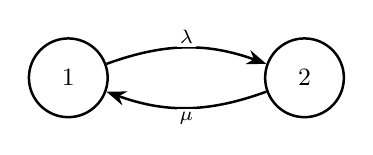
\begin{tikzpicture}[
    >=Stealth,
    line width=0.9pt,
    state/.style={circle, draw=black, minimum size=10mm, inner sep=0pt, font=\small},
    edge label/.style={font=\scriptsize, fill=white, inner sep=1pt}
]
    \node[state] (1) at (0,0) {$1$};
    \node[state] (2) at (3.0,0) {$2$};

    \draw[->, bend left=20] (1) to node[edge label, above] {$\lambda$} (2);
    \draw[->, bend left=20] (2) to node[edge label, below] {$\mu$} (1);
\end{tikzpicture}
\end{document}
